\title{Propuesta: Estructuras Abstractas de datos y Algoritmos/Proyecto c++}
%%%%%%%%%%%%%%%%%%%%%%%%%%%%%%%%%%%%%%%%%
% Journal Article
% LaTeX Template
% Version 1.3 (9/9/13)
%
% This template has been downloaded from:
% http://www.LaTeXTemplates.com
%
% Original author:
% Frits Wenneker (http://www.howtotex.com)
%
% License:
% CC BY-NC-SA 3.0 (http://creativecommons.org/licenses/by-nc-sa/3.0/)
%
%%%%%%%%%%%%%%%%%%%%%%%%%%%%%%%%%%%%%%%%%
%----------------------------------------------------------------------------------------
%       PACKAGES AND OTHER DOCUMENT CONFIGURATIONS
%----------------------------------------------------------------------------------------
\documentclass[paper=letter, fontsize=12pt]{article}
\usepackage[spanish]{babel} % English language/hyphenation
\usepackage{amsmath,amsfonts,amsthm} % Math packages
\usepackage[utf8]{inputenc}
\usepackage{float}
\usepackage{lipsum} % Package to generate dummy text throughout this template
\usepackage{blindtext}
\usepackage{graphicx}     % Para insertar gráficas
\usepackage{caption}
\usepackage{subcaption}
\usepackage[sc]{mathpazo} % Use the Palatino font
\usepackage[T1]{fontenc} % Use 8-bit encoding that has 256 glyphs
\linespread{1.05} % Line spacing - Palatino needs more space between lines
\usepackage{microtype} % Slightly tweak font spacing for aesthetics
\usepackage[top=25.4mm,left=25.4mm,right=25.4mm,bottom=25.4mm]{geometry}
\usepackage{multicol} % Used for the two-column layout of the document
%\usepackage[hang, small,labelfont=bf,up,textfont=it,up]{caption}
% Custom captions under/above floats in tables or figures
\usepackage{booktabs} % Horizontal rules in tables
\usepackage{float}
% Required for tables and figures in the multi-column environment -
% they need to be placed in specific locations
% with the [H] (e.g. \begin{table}[H])
\usepackage{hyperref} % For hyperlinks in the PDF
\usepackage{lettrine}
% The lettrine is the first enlarged letter at the beginning of the text
\usepackage{paralist}
% Used for the compactitem environment which makes bullet points with less space
% between them
\usepackage{abstract} % Allows abstract customization
\renewcommand{\abstractnamefont}{\normalfont\bfseries}
% Set the "Abstract" text to bold
\renewcommand{\abstracttextfont}{\normalfont\small\itshape}
% Set the abstract itself to small italic text
\usepackage{titlesec} % Allows customization of titles

\renewcommand\thesection{\Roman{section}} % Roman numerals for the sections
\renewcommand\thesubsection{\Roman{subsection}} % Roman numerals for subsections

\titleformat{\section}[block]{\large\scshape\centering}{\thesection.}{1em}{}
% Change the look of the section titles
\titleformat{\subsection}[block]{\large}{\thesubsection.}{1em}{}
% Change the look of the section titles
\newcommand{\horrule}[1]{\rule{\linewidth}{#1}}
% Create horizontal rule command with 1 argument of height
\usepackage{fancyhdr} % Headers and footers
\pagestyle{fancy} % All pages have headers and footers
\fancyhead{} % Blank out the default header
\fancyfoot{} % Blank out the default footer

\fancyhead[C]{
IE-0217: Estructuras Abstractas y Algoritmos
$\bullet$ Octubre 2015 $\bullet$ Propuesta }
% Custom header text

\fancyfoot[RO,LE]{\thepage} % Custom footer text
%-------------------------------------------------------------------------------
%       TITLE SECTION
%-------------------------------------------------------------------------------
\title{
\vspace{-15mm}\fontsize{24pt}{10pt}\selectfont\textbf{
Propuesta Proyecto Final:\\
Librería en C++ para generación automática de horaios en EIE}} % Article title
\author{
\large
{\textsc{Emilio Rojas, B15680}}\\[2mm]
{\textsc{Juan Sánchez, B16068}}\\[2mm]
{\textsc{Marco Montero, A94000}}\\[2mm]
{\textsc{}}\\[2mm]
\normalsize IE-0217: Estructuras Abstractas de datos y algoritmos\\[1mm]
% Your institution
\normalsize Escuela de Ingeniería Eléctrica \\ % Your institution
\normalsize Universidad de Costa Rica \\ % Your institution
\vspace{-5mm}
}
\date{}

%-------------------------------------------------------------------------------
\begin{document}
\maketitle % Insert title
\thispagestyle{fancy} % All pages have headers and footers
%\newpage
%\tableofcontents
%\newpage

\section{Introducción y Propuesta}
En la escuela de ingeniería eléctrica de la universidad de Costa Rica, el
proceso de asignación de horarios a los cursos se realiza de una forma
semi-automática por medio de una serie de hojas de datos en Excel, esto es útil
para el profesor encargado pero tiene ciertas fallas que podrían ser
solucionadas, además cabe destacar que el algoritmo puede ser implementado por
un lenguaje como C++ y optimizar así el proceso.

Un trabajo como este brindará una opción más automatizada que ayudará a agilizar
el proceso de creación de horarios, el cual es bastante laborioso en el estado
actual.

Además ayudará a los integrantes del proyecto a profundizar en conocimientos del
lenguaje de programación C++ y un inicio no despreciable en el uso de bases de
datos, ya que el gran bagaje del trabajo se basa en trabajar con los datos de
una base de datos que puede ser modificada según las necesidades semestrales de
la escuela.

%\section{Propuesta}

\section{Objetivos}

\subsection{General}
Implementar una librería en C++ con la capacidad de generar un horario de cursos
de acuerdo a los planes de estudio de escuela de ingeniería eléctrica de la
universidad de Costa Rica.

\subsection{Específicos}
\begin{itemize}
	\item Generar la estructura para una base de datos que contenga la
    información referente a profesores y cursos.
	\item Asignar a partir de la base de datos, profesores a los cursos tomando
    en cuenta limitaciones de horario de los mismos y cantidad de grupos por
    curso.
	\item Obtener un horario en el cual los cursos de cada bloque tenga al
    menos una posibilidad de ser matriculados todos sin que allá un traslape de
    horarios entre ellos.
\end{itemize}

\section{Planteamiento de la Solución}
La solución se basa en un diagrama de clases y en un diagrama de flujo, cuyo
proposito es explicar a un cierto nivel de abstracción como se pretende abarcar
el problema.

%\newpage
\subsection{Diagrama de Clases}

\begin{figure}[H]
  \centering
  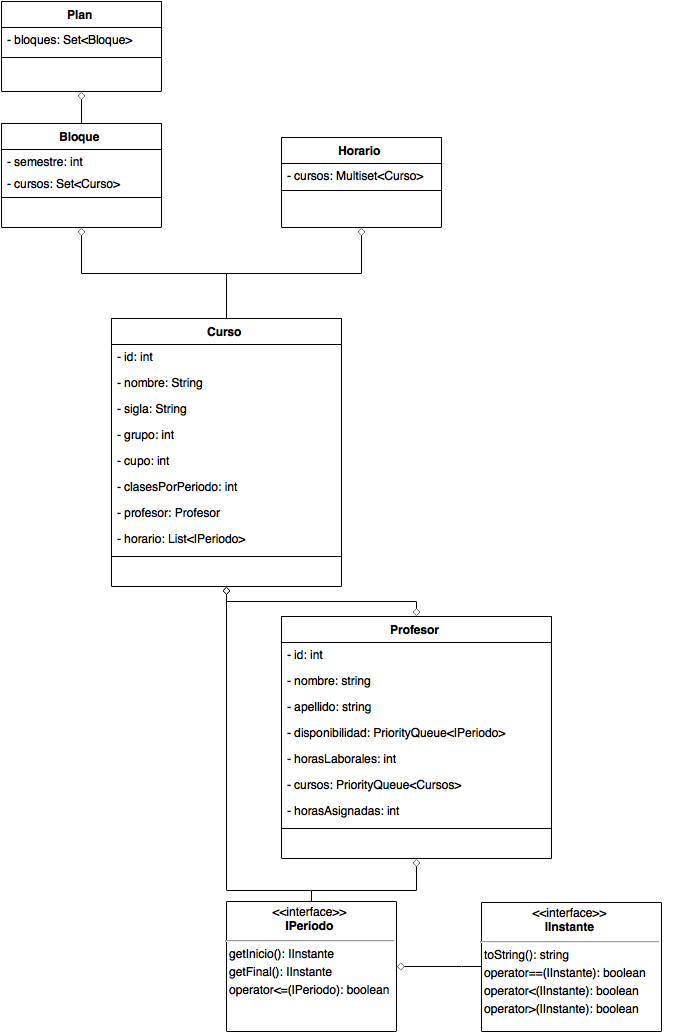
\includegraphics[scale=0.6]{HorariosCursos1.png}
\end{figure}

\begin{figure}[H]
  \centering
  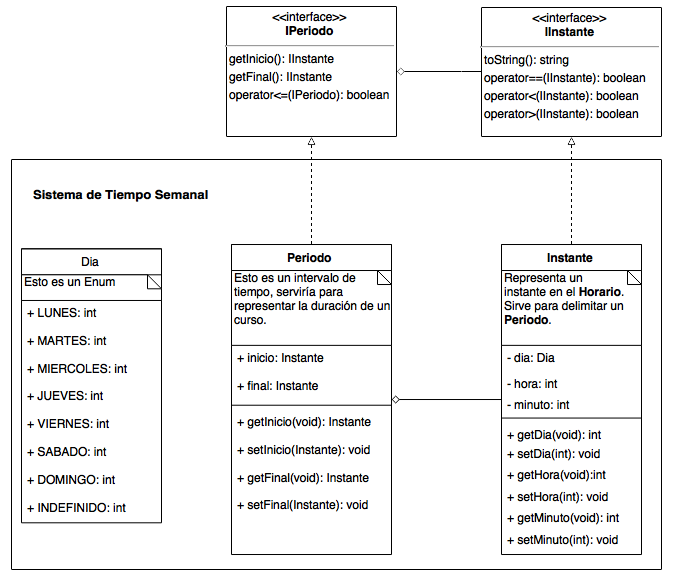
\includegraphics[scale=0.6]{HorariosCursos2.png}
  \caption{Diagrama de clases}
  \label{F:diaClases}
\end{figure}

El diagrama en \ref{F:diaClases} muestra las principales clases e interfaces que
se utilizarian para el desarrollo de la aplicación. La mayoría de las clases aún
no cuentan con métodos, esto se agregará en etapas posteriores del desarrollo.
Se muestran, sin embargo, los atributos de todas las clases, los cuales, se
pretende mantener a menos que surga la necesidad de añadir o eliminar atributos.
Similarmente, se han escogido algunas estructuras de datos(List, Set, Multiset,
etc) con poco criterio, por lo que quedan sujetas a cambios posteriores.

El sistema cuenta con planes, clase \texttt{Plan}, que representan un cierto
énfasis de la carrera, cada uno de estos planes, tiene asignados bloques, clase
\texttt{Bloque}, que vendría a ser el conjunto de cursos que propone el plan
para un dado semestre. Estas dos clases son bastante simples en su estructura,
y servirían para realizar chequeos de la viabilidad de un horario generado.

La clase \texttt{Horario} es la contenedora de un horario generado por la
libreria, y está compuesta únicamente por cursos. Los cursos que están
determinados por la clase \texttt{Curso}, que es una de las principales clases
del proyecto, esto porque contiene información relevante a las restricciones que
presenta el problema, como los profesores y el horario, que como se podrá
asumir, corresponden al profesor asignado y las horas y dias que se impartirá
cierto grupo de un curso. El profesor de un \texttt{Curso} se considera en la
clase \texttt{Profesor}, de cuyas características las más importantes son
\texttt{disponibilidad}, \texttt{horasLaborales} y \texttt{cursos}, que son las
limitantes de un profesor. La disponibilidad se refiere a las horas que podrían
asignarsele a un profesor, sin embargo no representan la cantidad horas que el
profesor labora, esto se representa con el número de \texttt{horasLaborales}.
Los \texttt{cursos} no representan los cursos que un profesor impartirá, sino
más bien los que este puede impartir.

Todo esto se basa en un sistema temporal representado por dos interfaces,
\texttt{IPeriodo} e \texttt{IInstante}. Un \texttt{IPeriodo}, tiene un
\texttt{IInstante} inicial y final. \texttt{IInstante} tiene únicamente
operaciones de relación, para indicar por ejemplo, si un momento es
\textit{mayor} a otro, siendo esto que el primero es posterior.
Debido a la naturaleza de los horarios a crear, se utilizará un sistema
de tiempo semanal, con 7 días  y uno indefinido, que se utiliza para designar
horas en un día cualquiera. Además se contemplan las horas y minutos de cada
día.

\subsection{Diagrama de Flujo}
El diagrama de flujo del algoritmo se puede observar en la figura \ref{F:flujo}.
Su recorrido básico será el siguiente:

\begin{enumerate}
    \item En primera instancia se elige un énfasis para el plan (\textbf{W}).
    \item Si el valor está dentro de rango (de 1  a 3) se eligé un bloque dentró
    del plan (\textbf{j}).
    \item Se elige un curso dentro del plan (\textbf{i}).
    \item Se procede a buscar un profesor para asignar al curso elegido.
    \item Si se no se asigna profesor al curso, se añade a una lista de
    excepciones (cursos en conflicto).
    \item Si se hace match entre un curso y un horario de un profesor, se
    elimina el horario asignado de las posibilidades de horario dentro del
    bloque.
    \item Luego se pasa al siguiente curso del plan.
    \item Una vez que se completa el bloque se pasa al siguiente dentro del
    plan.
    \item Una vez que se recorre todo el plan, se pasa al siguiente.
    \item Si se recorrieron todos los planes de estudio, termina de ejecutar.
\end{enumerate}

\begin{figure}[H]
\centering
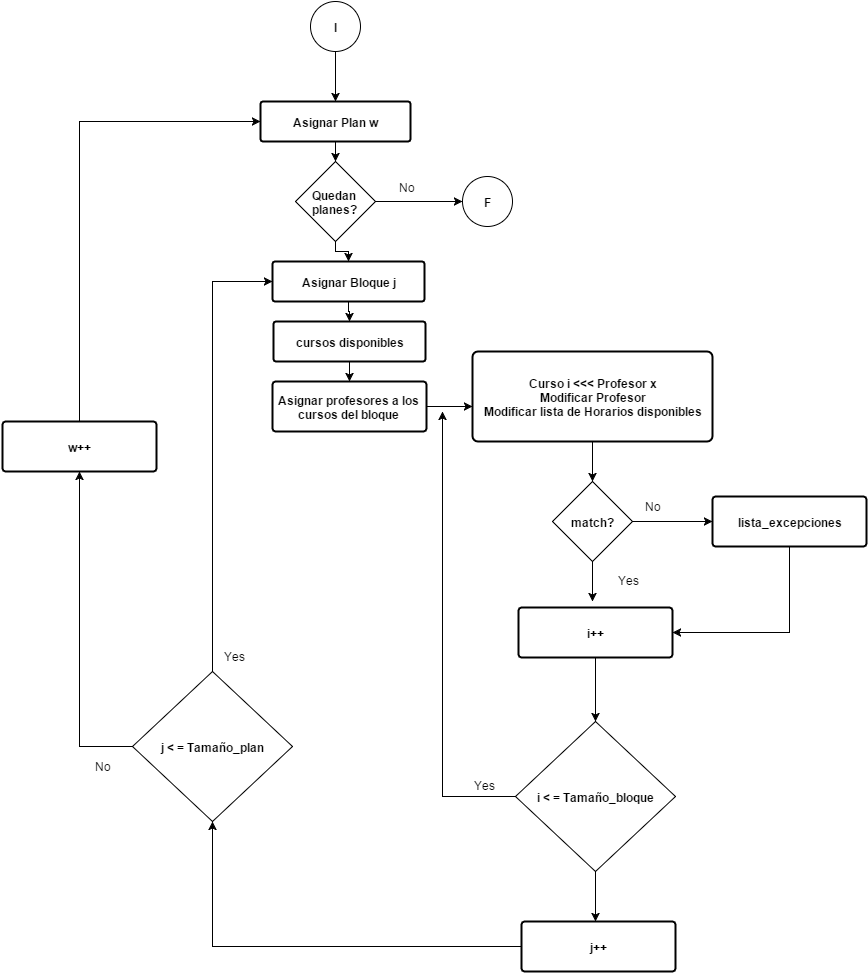
\includegraphics[width=1\textwidth]{flujo.png}
\caption{Diagrama de Flujo para el algoritmo}
\label{F:flujo}
\end{figure}

\section{Aspectos a Considerar}
Respecto al manejo del proyecto, se tiene previsto el manejo de actividades
según el diagrama de Gantt mostrado en la figura \ref{F:gantt}. En primera
instancia se planea realizar entre los 3 miembros de equipo  un estudio
preeliminar de manejo para la base de dato. \\
Paralelo a esto se desarrollará la recolección de datos para la creación de la
base de datos  en \textbf{mySQL}.

\begin{figure}[H]
    \centering
    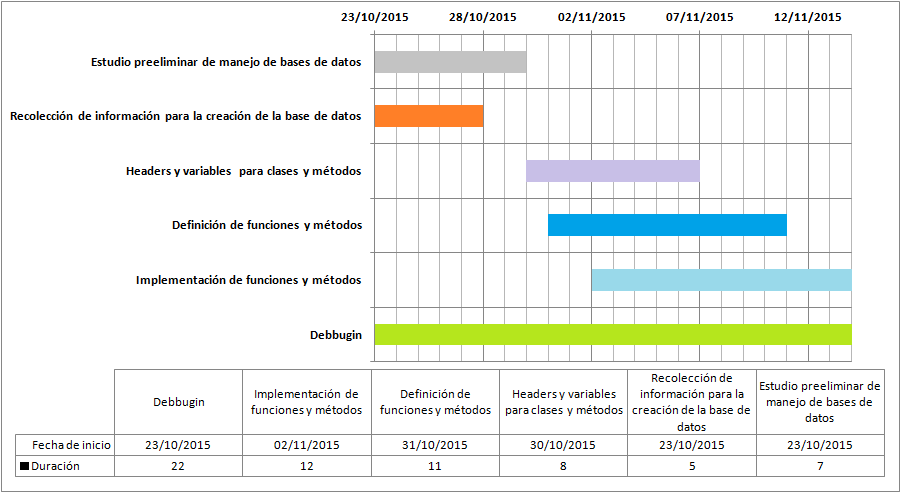
\includegraphics[width=0.9\textwidth]{ganttcolor.png}
    \caption{Diagrama de Gantt propuesto para el proyecto }
    \label{F:gantt}
\end{figure}

La recolección de datos se realizará entre los 3 miembros de ser necesario y
Emilio se encargará de la elaboración de la base de datos.\\
Posteriormente, entre Juan y Marco iniciaran la creación de los headers para
las clases y métodos. Una vez se tenga lista la base de datos, Emilio se
integrará a el proceso de definicón de funciones e implementación junto con el
resto del equipo. \\
Paralela a todas las demás tareas, se mantendrá un constante proceso de
debbugin en el proyecto. Este a cargo de todos los mismbros del equipo.

\end{document}
